\documentclass[10pt, a4paper]{article}
\usepackage[francais]{babel}
\usepackage[utf8]{inputenc}
\usepackage[T1]{fontenc}
\usepackage{hyperref}
\usepackage[]{graphicx}
\usepackage{url}
\usepackage[a4paper, left=2.5cm, right=2.5cm, top=2.0cm, bottom=2.0cm, headsep=1.0cm]{geometry}
\usepackage{subfigure}
\usepackage{epstopdf}

\setcounter{totalnumber}{5}
\renewcommand{\topfraction}{0.9}
\renewcommand{\bottomfraction}{0.9}
\newcommand{\linia}{\rule{\linewidth}{0.4mm}}

\newtheorem{mydef}{Definition}

\author{Yann Colin \\Grzegorz Maj}
\title{Médiatheque}

\makeatletter
\def\maketitle{%
\begin{titlepage}
	\begin{center}
		\LARGE
		\textsc{Compte rendu \\ Projet Informatique}
	\end{center}

	\vspace{3cm}

	\begin{center}\leavevmode
      \hrule
    \vskip 1pt
	\linia
	\vskip 0.5cm
	\Huge \textsc{\@title}\par

	\vskip 0.5cm
      	\linia
      \vskip 1pt
      \hrule

	\vskip 2mm

	\vspace{1.5cm}
	\begin{flushright}
		\begin{minipage}{5cm}
			\textit{\normalsize Auteurs:}\\
			\Large \textit{\@author} \par
			\vskip 2pt
			\hrule
			
		\end{minipage}
	\end{flushright}
    

	\end{center}%
	\vspace*{\stretch{6}}
    \begin{center}
    10 janvier 2016
    \end{center}
\end{titlepage}
	}
\makeatother



\begin{document}
\bibliographystyle{plain}
    \maketitle
    
    \tableofcontents
    \newpage
    
     \section{La conception}
     
	     \subsection{Diagramme UML}
	     
	     \begin{figure}[h]
			\begin{center}
				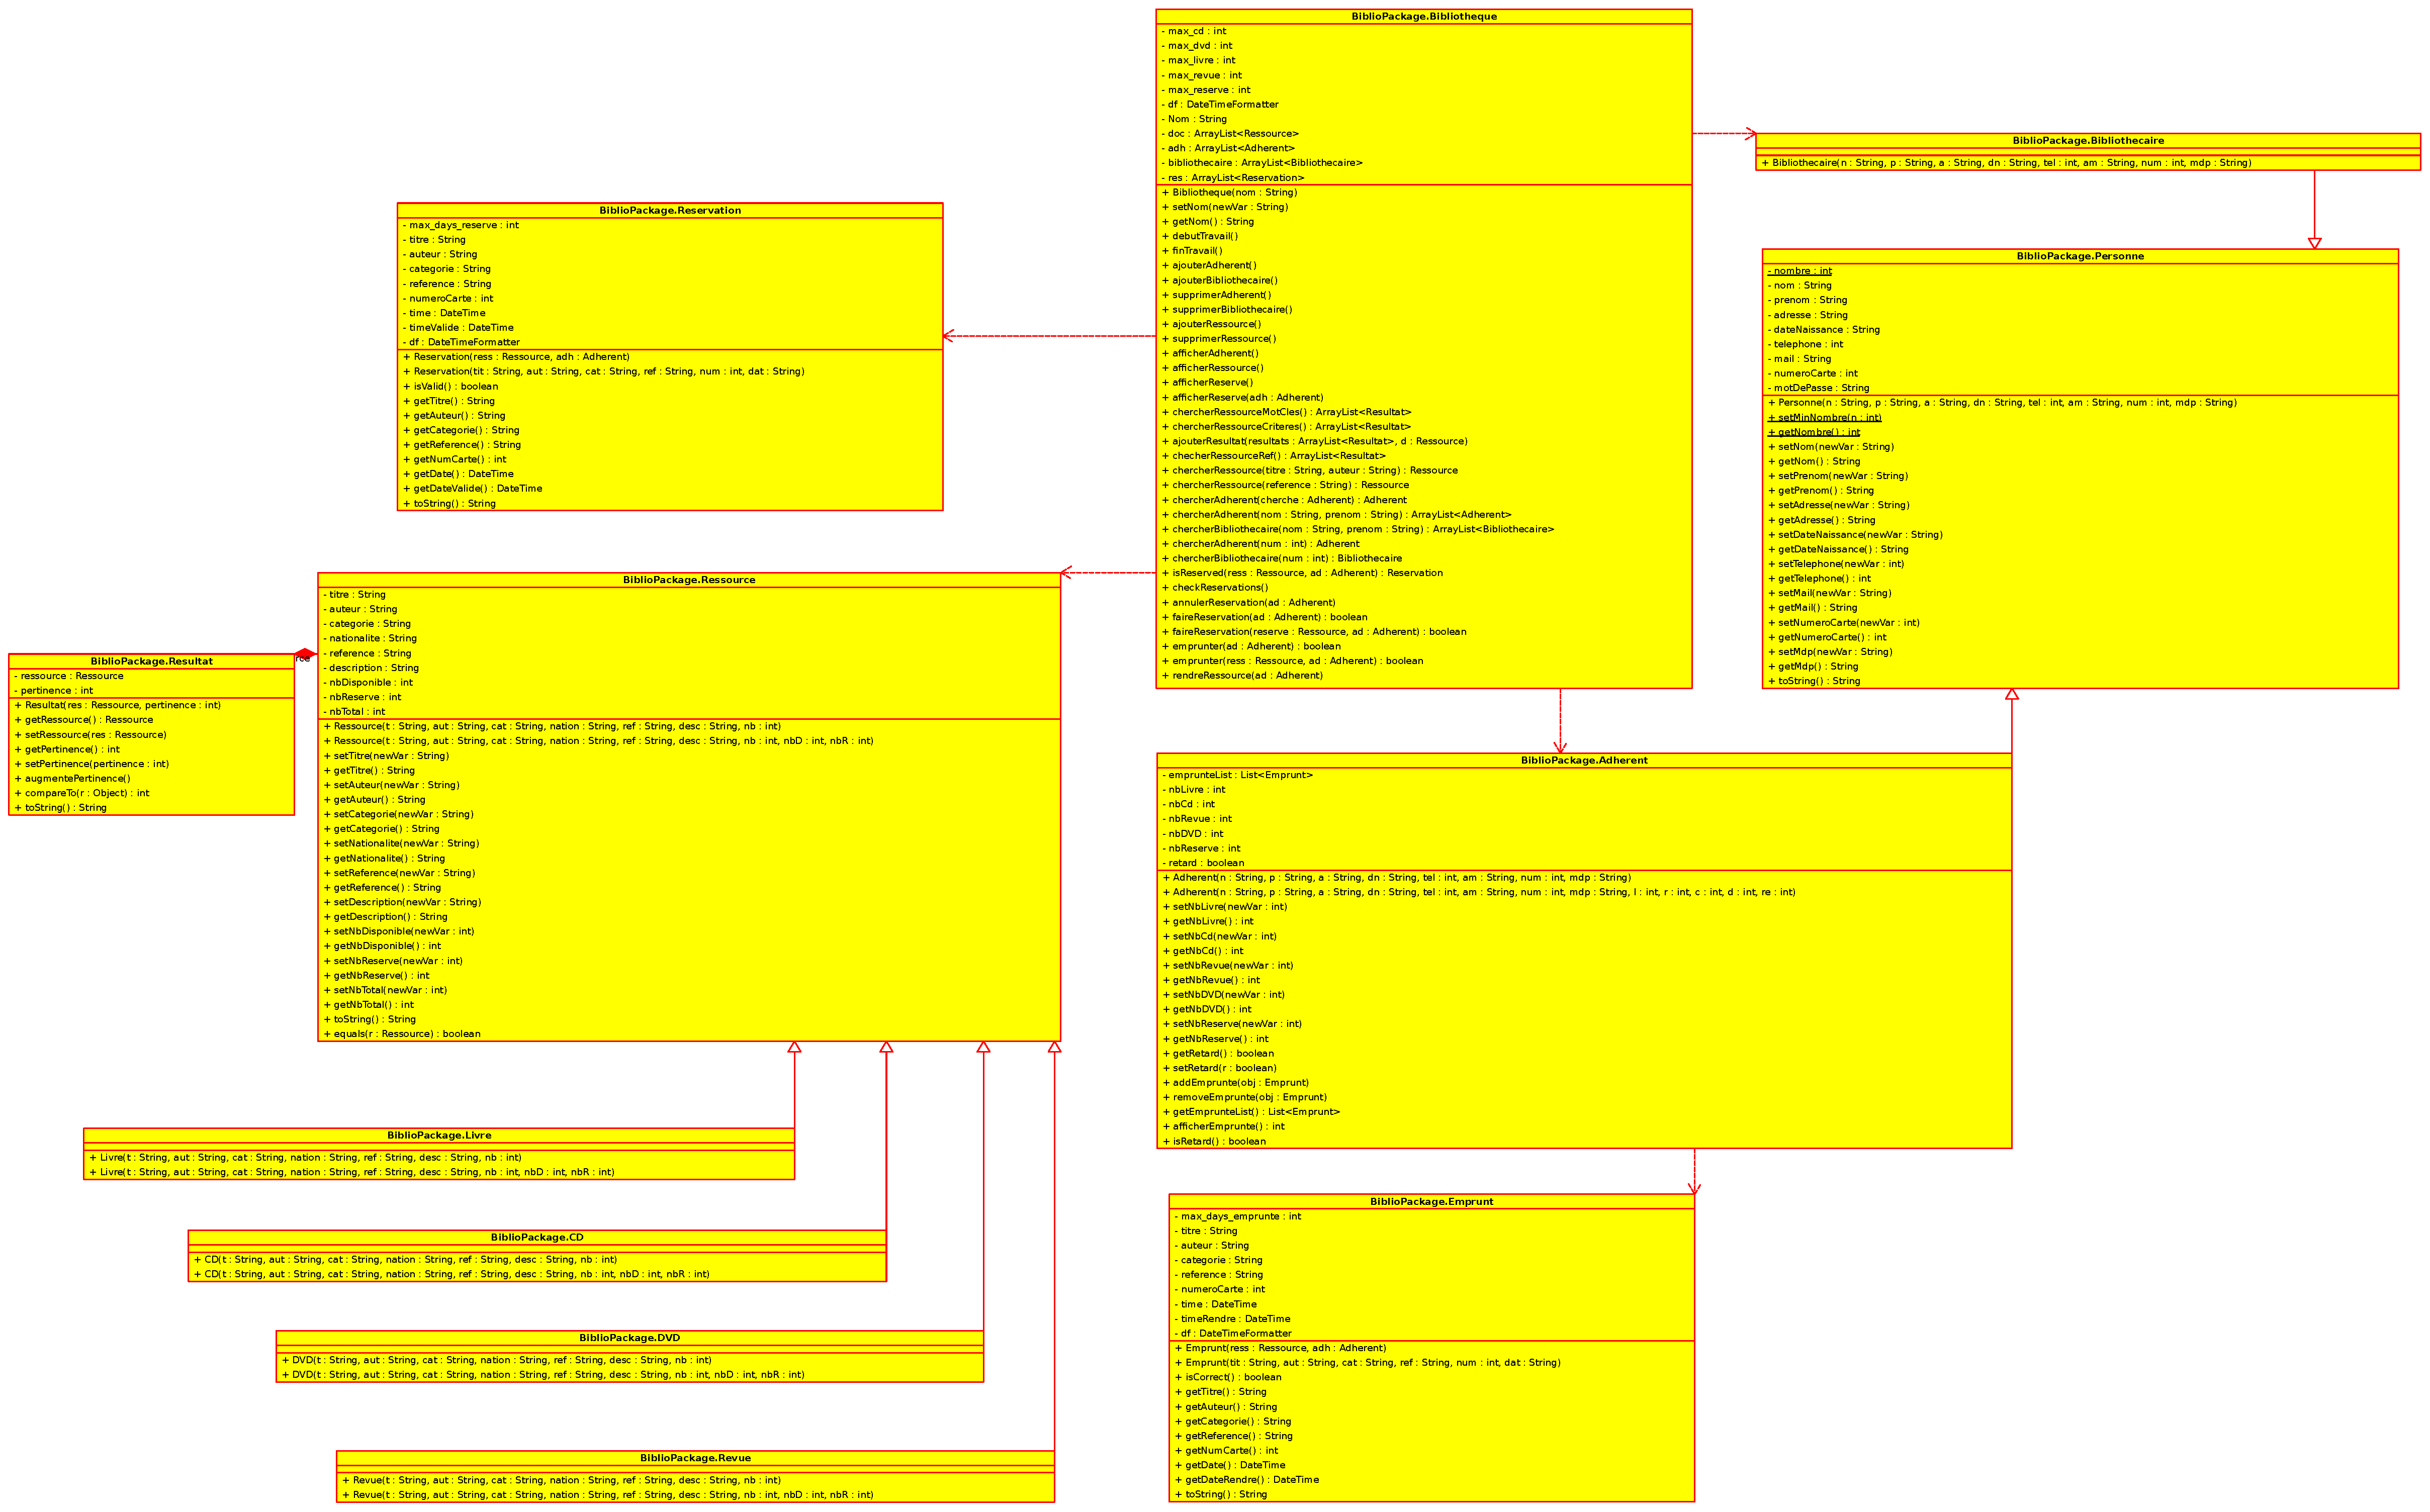
\includegraphics[width=1\textwidth]{graphics/class.eps}
				\caption{Diagramme UML de classes.}
			\end{center}
		\end{figure}
     
    		 \subsection{Cas d'utilisation}
    		 
    		 \begin{figure}[h]
			\begin{center}
				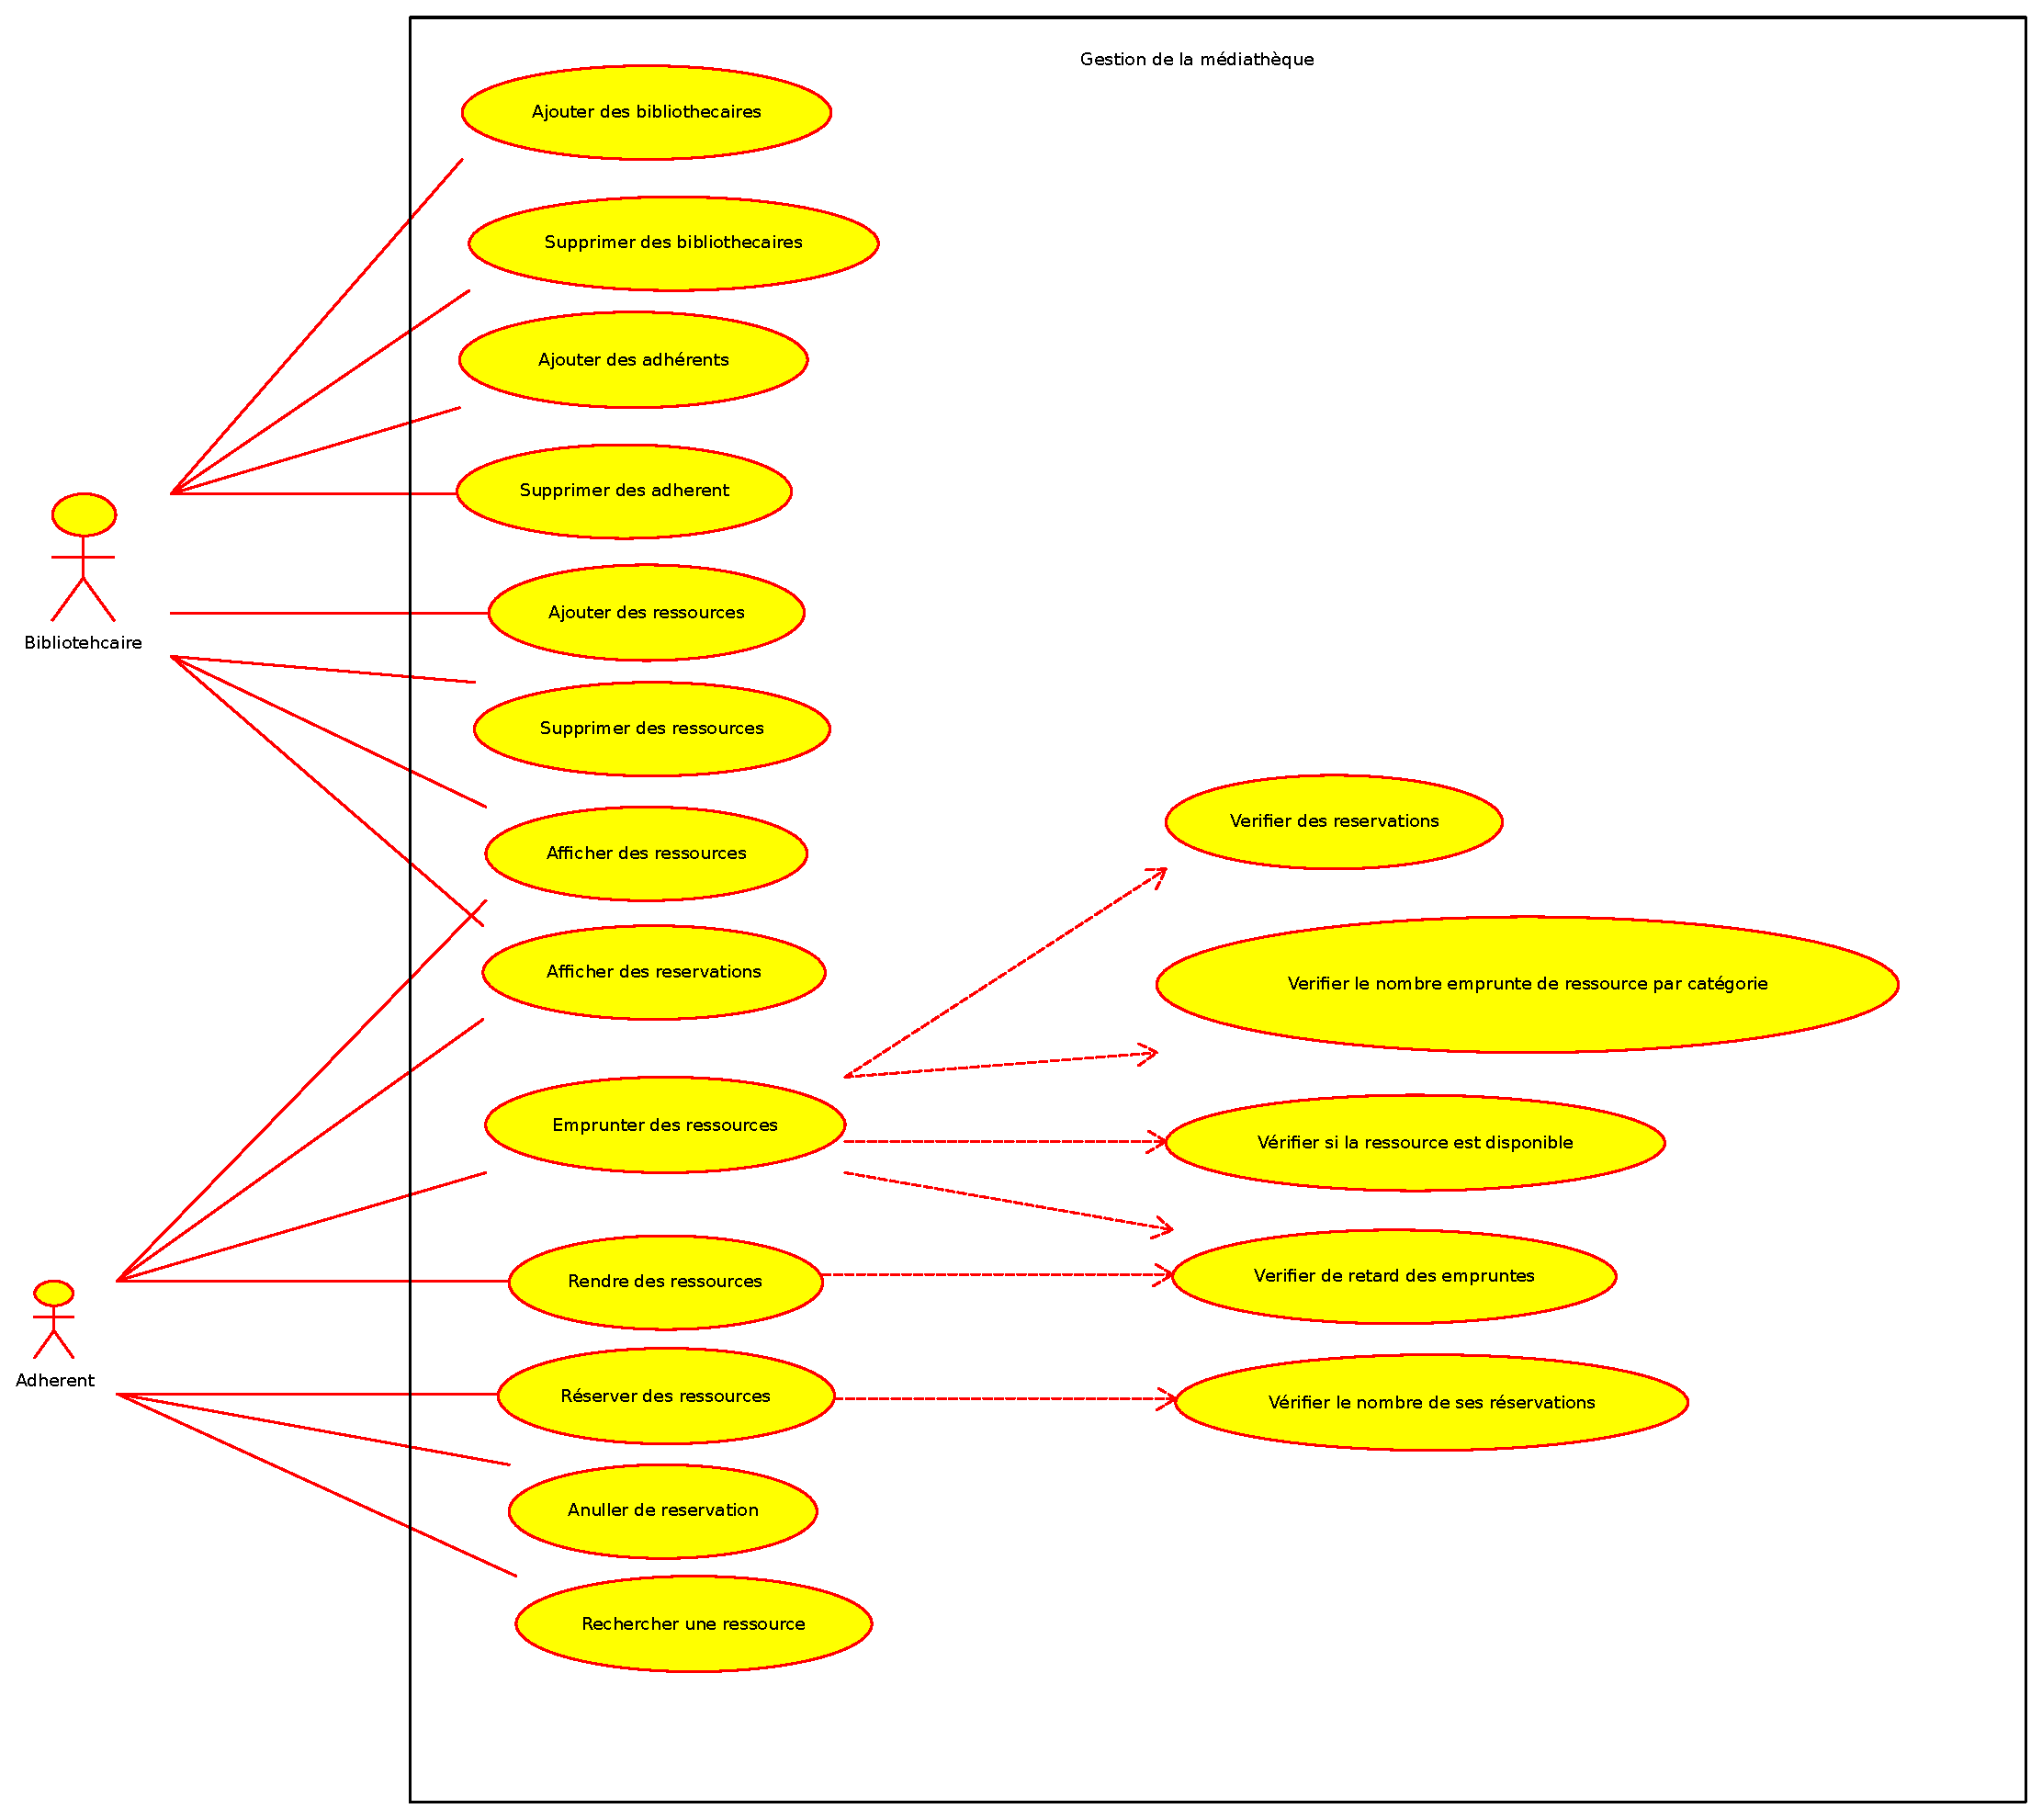
\includegraphics[width=1\textwidth]{graphics/usecasediagram.eps}
				\caption{Diagramme cas d'utilisation.}
			\end{center}
		\end{figure}
	
	\section{Implémentation}
	
	\section{Les tests}
	
	\section{Façon de travail}
		\subsection{Partage de travail}
		
		
		\subsection{Logiciel de gestion de version}
		Git et serveur GitHub		
		
		\subsection{Les problèmes}
		
		
	

\bibliography{bibliografia.bib}

\end{document}
